\chapter{Evaluation}
\label{chap:evaluation}
In this chapter, we evaluate different aspects of the developed system. Section \ref{sec:cost_and_performance} shows a cost and a performance analysis of the developed \gls{sc}. Section \ref{sec:field_test} concludes the analyses with a field test of a simulated artwork transportation scenario. Finally, this chapter is concluded with a discussion in Section \ref{sec:eval_discussion} To evaluate the performance of the system we also recorded the response time of each request. This can give an indicator

\section{Cost and Performance Analysis}
\label{sec:cost_and_performance}
The primary cost factor of the artis-system is the \gls{sc}. Each execution of a function that mutates the state of the \gls{sc} costs a certain amount of gas which in turn has a price in Ether. The cost for a transaction thus is calculated as follows:
$$
transaction\ fee = gas \times gas\ price
$$
To analyze the execution costs of the \textit{safeMint} and \textit{updateArtworkData} contract functions, we executed the corresponding requests of the developed \gls{api} multiple times $(n = 10)$ for each input variety. This analysis was conducted on the sepolia testnet and the resulting transactions were inspected on the Etherscan block explorer. The transactions were submitted with a relatively high gas price (30 Gwei) to make the transactions attractive for validators \cite{ethergas}. During this analysis, we observed that the gas used for a specific function depends on the input parameters but does not vary if the input parameters are the same. To analyze the performance, we also recorded the processing time of each request. This time can be an indicator of the performance but depends on the state of the blockchain and likely differs on the mainnet.

To get a sense of how gas translates into fees, we used the average gas price of the past month for the Ethereum mainnet (28 Gwei, 07.08.23 - 08.08.23) \cite{gaspriceaverageethereum} and the current value of Ether in \gls{chf} (1625.20 CHF = 1 ETH, 09.08.23) \cite{coinmarketcap}. Because the contract can also be deployed on other blockchains that use the \gls{evm}, we decided to include the cost on the polygon network. Except the contract has not been deployed to the Polygon network, and the same amount of gas was used for these calculations. The average gas price of the past month (173 Gwei \cite{gaspriceaveragepolygon}, 07.08.23 - 08.08.23) was multiplied by the gas and converted into \gls{chf} by using the current price for MATIC (0.60 CHF = 1 MATIC, 09.08.23) \cite{coinmarketcap}. The results were rounded to four decimal points for the tokens and two decimal points for \gls{chf}.

\begin{figure}[ht]
    \begin{subfigure}{0.49\textwidth}
        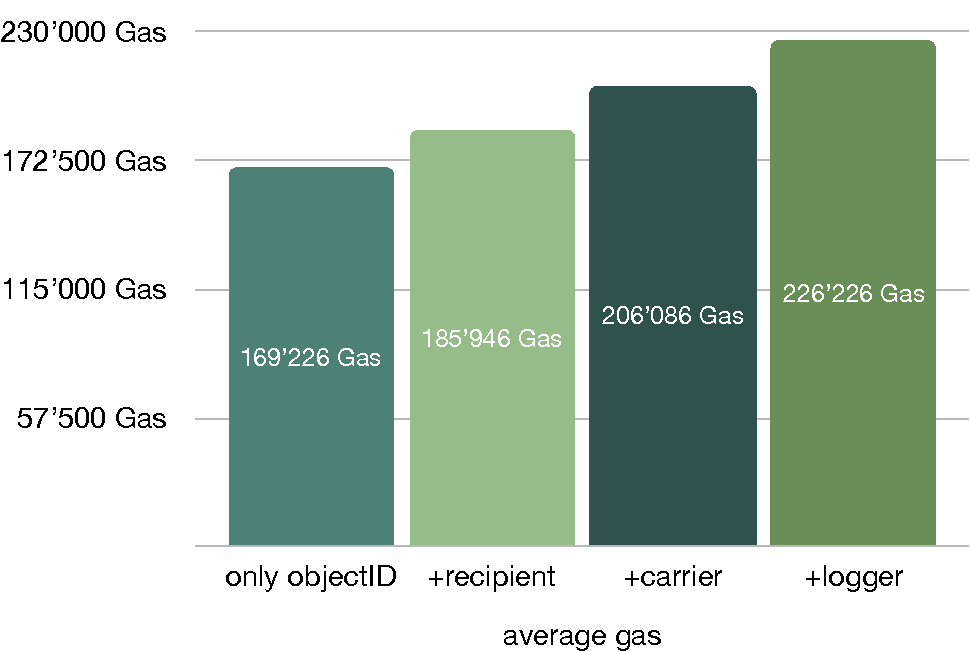
\includegraphics[width=\textwidth]{diagrams/safeMint_gas_eval.pdf}
        \caption{Transaction gas usage}
        \label{fig:safemint_tx_cost}
    \end{subfigure}
    \hfill
    \begin{subfigure}{0.49\textwidth}
        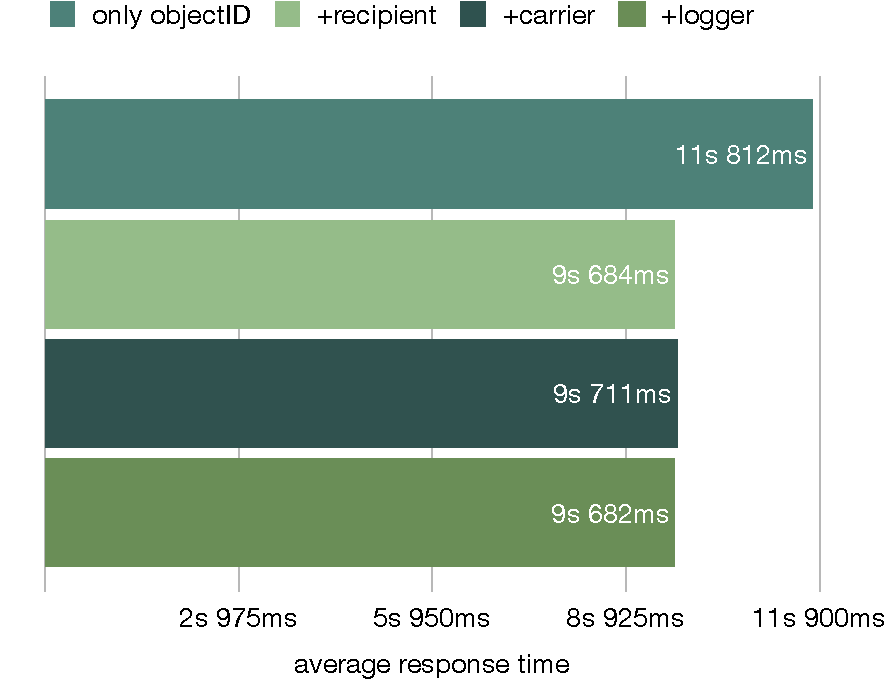
\includegraphics[width=\textwidth]{diagrams/safeMint_request_time_eval.pdf}
        \caption{Request speed in seconds}
        \label{fig:safemint_tx_speed}
    \end{subfigure}
    \caption{safeMint analysis}
    \label{fig:safemint_analysis}
\end{figure}

\subsection*{safeMint}
Figure \ref{fig:safemint_tx_cost} shows the average gas the safeMint function consumes for various input parameters. Each bar shows the average of 10 function executions. The very left bar shows the average gas used if only the objectID of the artwork is added during minting. The second bar shows the gas consumed if the objectID and the recipient address are provided during minting. This pattern remains the same for the last two bars. The analysis shows that the more parameters are provided, the more gas it consumes. Table \ref{tab:safemint_tx_fees} shows the transaction fees in the corresponding native token and converted into \gls{chf} as outlined above. 

\begin{table}[h]
\begin{adjustbox}{width=1\textwidth}
\begin{tabular}{cllll}
\multicolumn{1}{l}{}                                                           & \textbf{only objectID} & \textbf{+recipient} & \textbf{+carrier} & \textbf{+logger} \\ \hline 
\textbf{\begin{tabular}[c]{@{}c@{}}transaction fee\\ ETH (MATIC)\end{tabular}} & 0.0048 (0.0293)        & 0.0053 (0.0322)     & 0.0059 (0.0357)   & 0.0064 (0.0392)  \\ \hline
\textbf{\begin{tabular}[c]{@{}c@{}}in CHF \\ Ethereum (Polygon)\end{tabular}}  & 7.83 (0.02)            & 8.61 (0.02)         & 9.54 (0.02)       & 10.47 (0.02)    
\end{tabular}
\end{adjustbox}
\caption{Estimated transaction fees safeMint}
\label{tab:safemint_tx_fees}
\end{table}

The response time of the \gls{api} calls are mostly below 10s. We could not observe a large difference in the different input parameters. The chart in Figure \ref{fig:safemint_tx_speed} shows the average response time in seconds. The maximum response time recorded was 33s on the fifth call with only the objectID submitted, and the minimum was 3s with the objectID and recipient address submitted. This shows that this metric can fluctuate heavily depending on the state of the network.

\begin{figure}[ht]
    \begin{subfigure}{0.49\textwidth}
        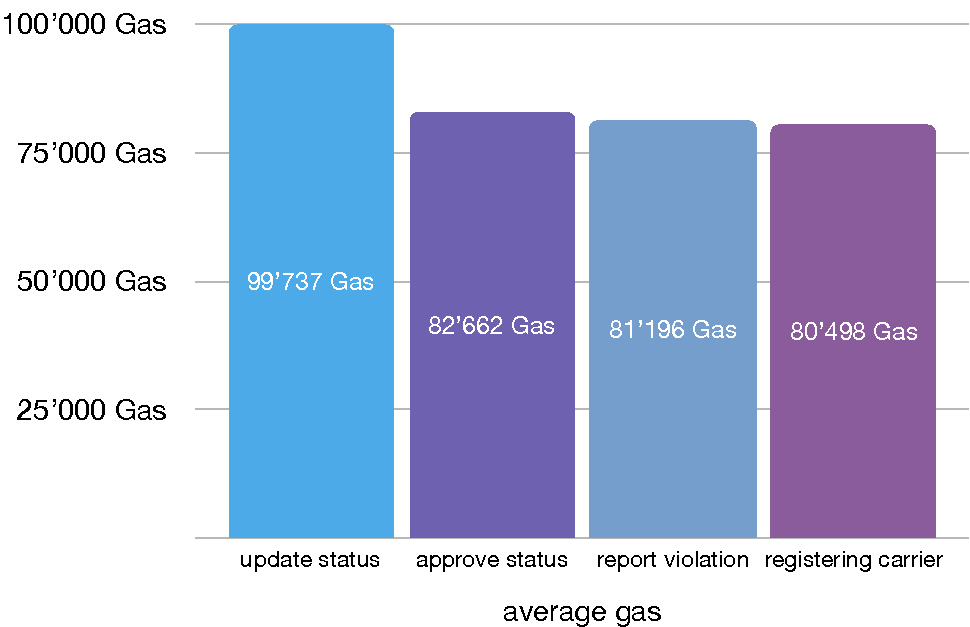
\includegraphics[width=\textwidth]{diagrams/updateArtworkData_gas_eval.pdf}
        \caption{Transaction gas usage}
        \label{fig:updateArtworkData_tx_cost}
    \end{subfigure}
    \hfill
    \begin{subfigure}{0.49\textwidth}
        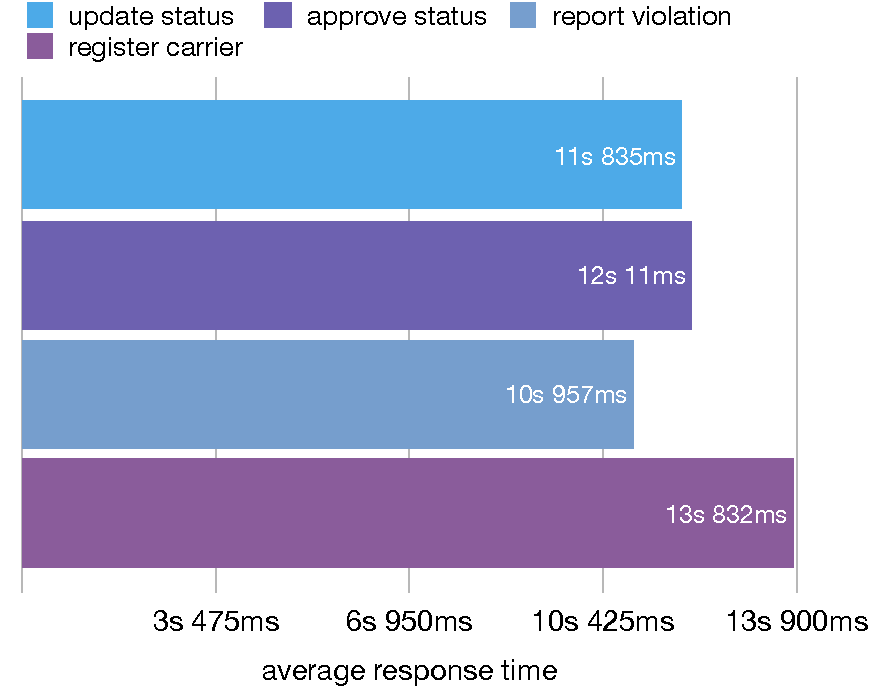
\includegraphics[width=\textwidth]{diagrams/updateArtworkData_request_time_eval.pdf}
        \caption{Request speed in seconds}
        \label{fig:updateArtworkData_tx_speed}
    \end{subfigure}
    \caption{updateArtworkData analysis}
    \label{fig:updateArtworkData_analysis}
\end{figure}

\subsection*{updateArtworkData}
Similarly, we also analyzed the updateArtworkData function. The bar on the very left of Figure \ref{fig:updateArtworkData_tx_cost} shows the average gas consumed by the function when updating the requested status. Approving the status as a different actor shows an average gas consumption of 82'662. The last two bars show the gas amount for reporting a violation from the logger and registering a carrier.

The cost of these transactions was estimated similarly to with the safeMint function (Table \ref{tab:updateArtworkData_tx_fees}). The results show that updating an artwork \gls{nft} is much less costly than minting it. 

\begin{table}[h]
\begin{adjustbox}{width=1\textwidth}
\begin{tabular}{cllll}
\multicolumn{1}{l}{}                                                           & \textbf{update status} & \textbf{approve status} & \textbf{report violation} & \textbf{register carrier} \\ \hline 
\textbf{\begin{tabular}[c]{@{}c@{}}transaction fee\\ ETH (MATIC)\end{tabular}} & 0.0028 (0.0173)        & 0.0024 (0.0143)     & 0.0023 (0.0141)   & 0.0023 (0.014)  \\ \hline
\textbf{\begin{tabular}[c]{@{}c@{}}in CHF \\ Ethereum (Polygon)\end{tabular}}  & 4.62 (0.01)            & 3.83 (0.01)         & 3.76 (0.01)       & 3.73 (0.01)    
\end{tabular}
\end{adjustbox}
\caption{Estimated transaction fees updateArtworkData}
\label{tab:updateArtworkData_tx_fees}
\end{table}

The average response time of updating an \gls{nft} varies depending on the input parameters. The request that was fulfilled the fasted approved a status change in around three Seconds. Interestingly, the longest response time of over 35 seconds was recorded on the same type of request.


\subsection*{Non-Mutating Functions}
The GET endpoints exposed by the \gls{api} target several functions that do not mutate the state of the \gls{sc}. These functions do not cost gas, and their execution time is much less (usually < 1 Second). Additionally, the artis-server adds a caching layer to these function calls, which generally reduces the response time of repeated calls to a few milliseconds.

\section{Security Analysis}
\label{sec:security_analysis}
Since the system is intended to be used by different actors in a trust-less environment a security analysis is vital for evaluating the prototype. The following section discusses the different attack surfaces and evaluates the security risk.

\subsection{Threat Scenarios}
% You can improve the analysis here by considering those aspects in terms of CIA (Confidentiality, Integrity, and Availability). 
% Even a small table with risk assessment 
\subsubsection{Compromised Logger}
The logging device is important to the system, and a compromised device would lead to a compromised system altogether. We consider three different attack scenarios when it comes to the logger.
\subsubsection{Software Exploitation}
Currently, the device itself is not secured in any way. Any malicious actor could connect to the logger device and alter its software. This could include changing the violation thresholds, stopping the logging script, manipulating the local database of the readings, and more. The current system is not protected against this threat, and thus, the security risk is high.
\subsubsection{Hardware Exploitation}
The recordings can also be influenced externally by exploiting the hardware components. By gaining access to the logger device, a malicious actor could influence the environmental parameters in a minimal perimeter around the sensor and falsify the readings. This could result in violations even if the artwork itself was not affected or could prevent violations even if the artwork was affected. The current system is not protected against this threat, and the security risk is high.
\subsubsection{Compromised Credentials}
The system only allows registered actors to change the \gls{nft}. This is also true for the logger device, which authenticates the system by signing a challenge message with a private key. If the private key is leaked, a malicious actor could report violations even if none occurred. Currently, the private key is stored in an environment variable on the software. An attacker could easily retrieve the value of the private key by connecting to the logger. This indicates a high-security risk for this threat.

\subsection{Compromised Smart Contract}
A malicious actor could influence the state of the \gls{sc} by accessing it directly. The attacker would have to identify flaws in the contract code and find an exploit to manipulate artwork data. We estimate the security risk of finding a flaw in the code to be medium, as the contract was tested during development, and basic code-checking tools could not identify a vulnerability. The \gls{sc} only accepts transactions issued by the system's admin. If the admin credentials are leaked, the attacker would have unlimited access to the \gls{sc}. In the current system, the admin's private key is only stored on the artis-server. The server is deployed as a Google Cloud-run service, and the Google secret manager supplies the private key. The security risk for this threat scenario is estimated to be low because the secret manager is an industry-standard solution for managing sensitive data.

\subsection{Disclosure of Data}
The data stored on the \gls{sc} could be sensitive depending on the use case. The \gls{sc} prevents unauthorized users from reading data. However, the transactions submitted to update data can contain sensitive information. This information can be read by anyone that has access to the \gls{sc} address, admin address, or any of the actors' addresses. Because these addresses are not considered secrets, the system must disclose all data to the public. This could introduce a high-security risk for certain use cases.

\section{Field Test}
\label{sec:field_test}
Because the isolated analyses performed above do not indicate how the system would perform during an artwork transportation scenario, we used the system on a simulated transportation scenario.

\begin{figure}[ht]
    \centering
    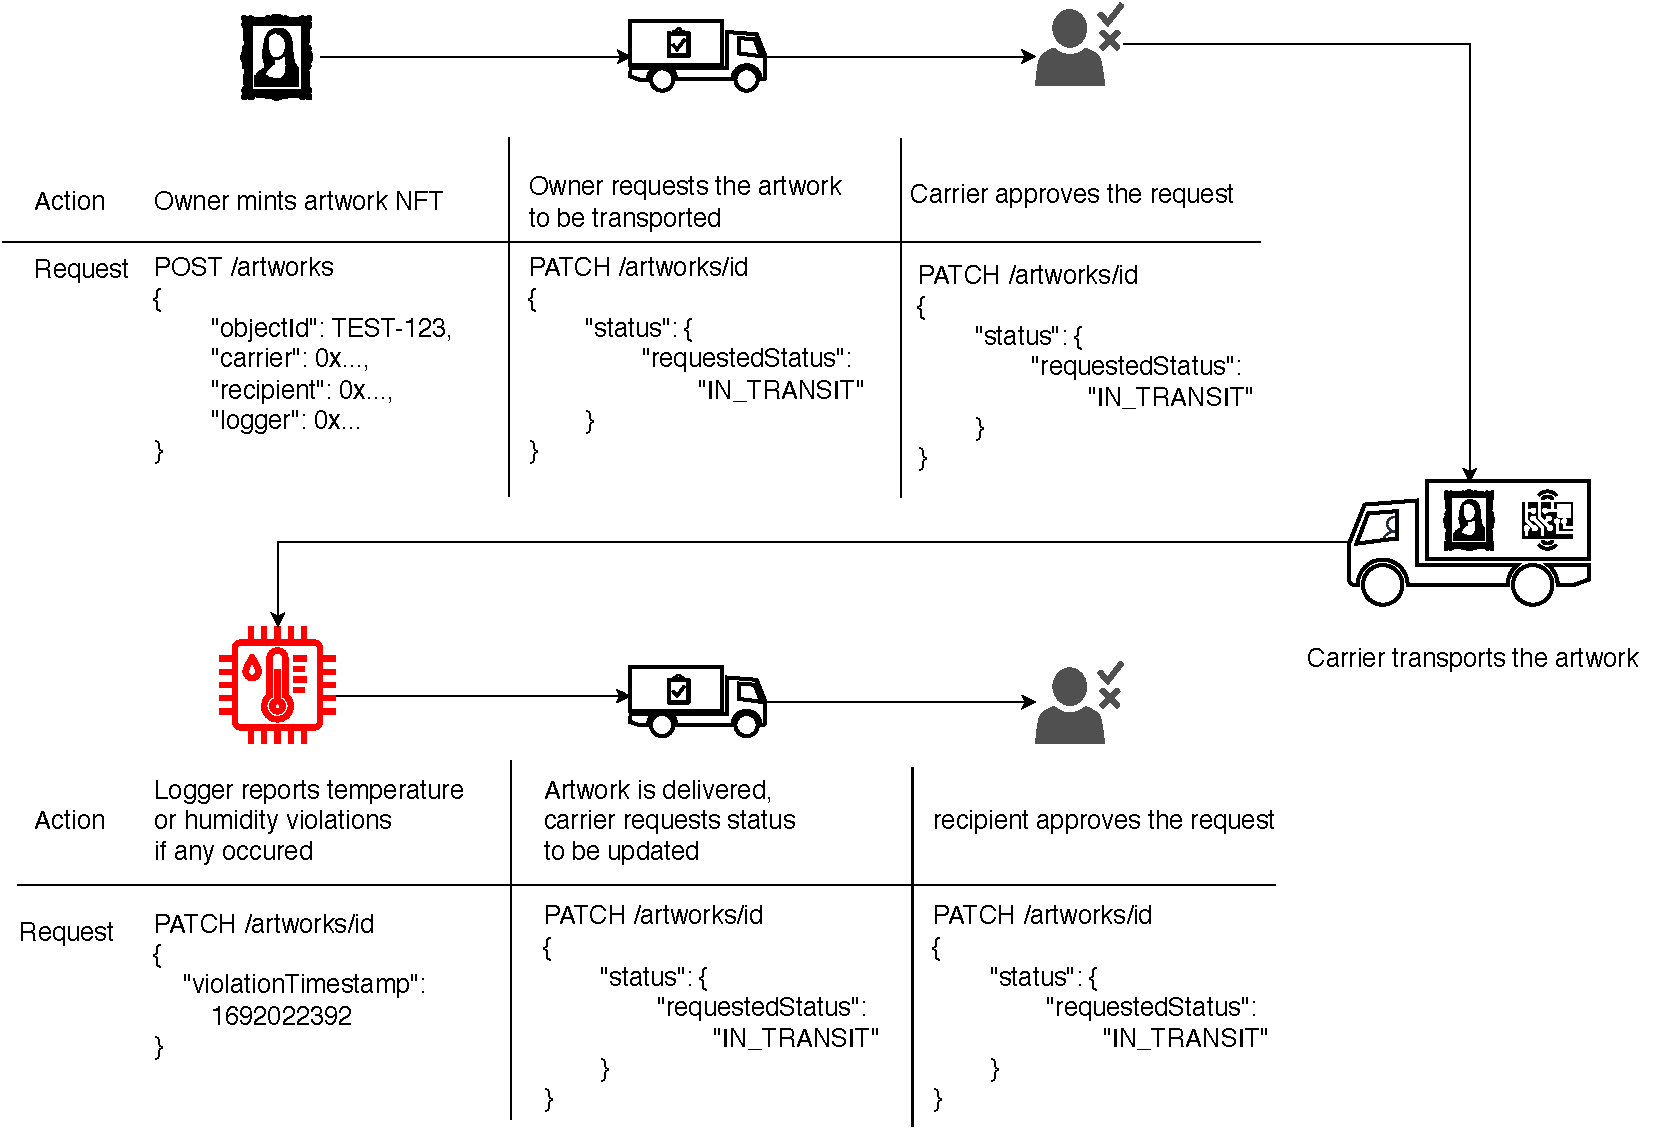
\includegraphics[width=0.9\textwidth]{diagrams/evaluation_scenario_v2.drawio.pdf}
    \caption{Field test scenario}
    \label{fig:eval_scenario}
\end{figure}

The steps of the simulated scenario are visualized in Figure \ref{fig:eval_scenario} and described in more detail below.

\begin{enumerate}
    \item Creates a new artwork \gls{nft} and registers the corresponding roles using the artis-frontend.
    \item Request the status of the artwork to be changed to \textit{IN\_TRANSIT} from the sender account
    \item Approve this request from the carrier account
    \item Enable the logger by starting the \textit{logging\_script} and the \textit{violation\_script} with the thresholds of 25 degrees Celcius and 70\% humidity.
    \item Take the logging device and transport it from the point of departure to the destination
    \item During the transportation, simulate a violation by wrapping a hand around the sensor to increase the temperature.
    \item Upon arrival, request the status of the artwork to be changed to \textit{DELIVERED} from the carrier account
    \item Approve this request from the recipient account
\end{enumerate}

\begin{figure}[ht]
    \begin{subfigure}{0.5\textwidth}
        \centering
        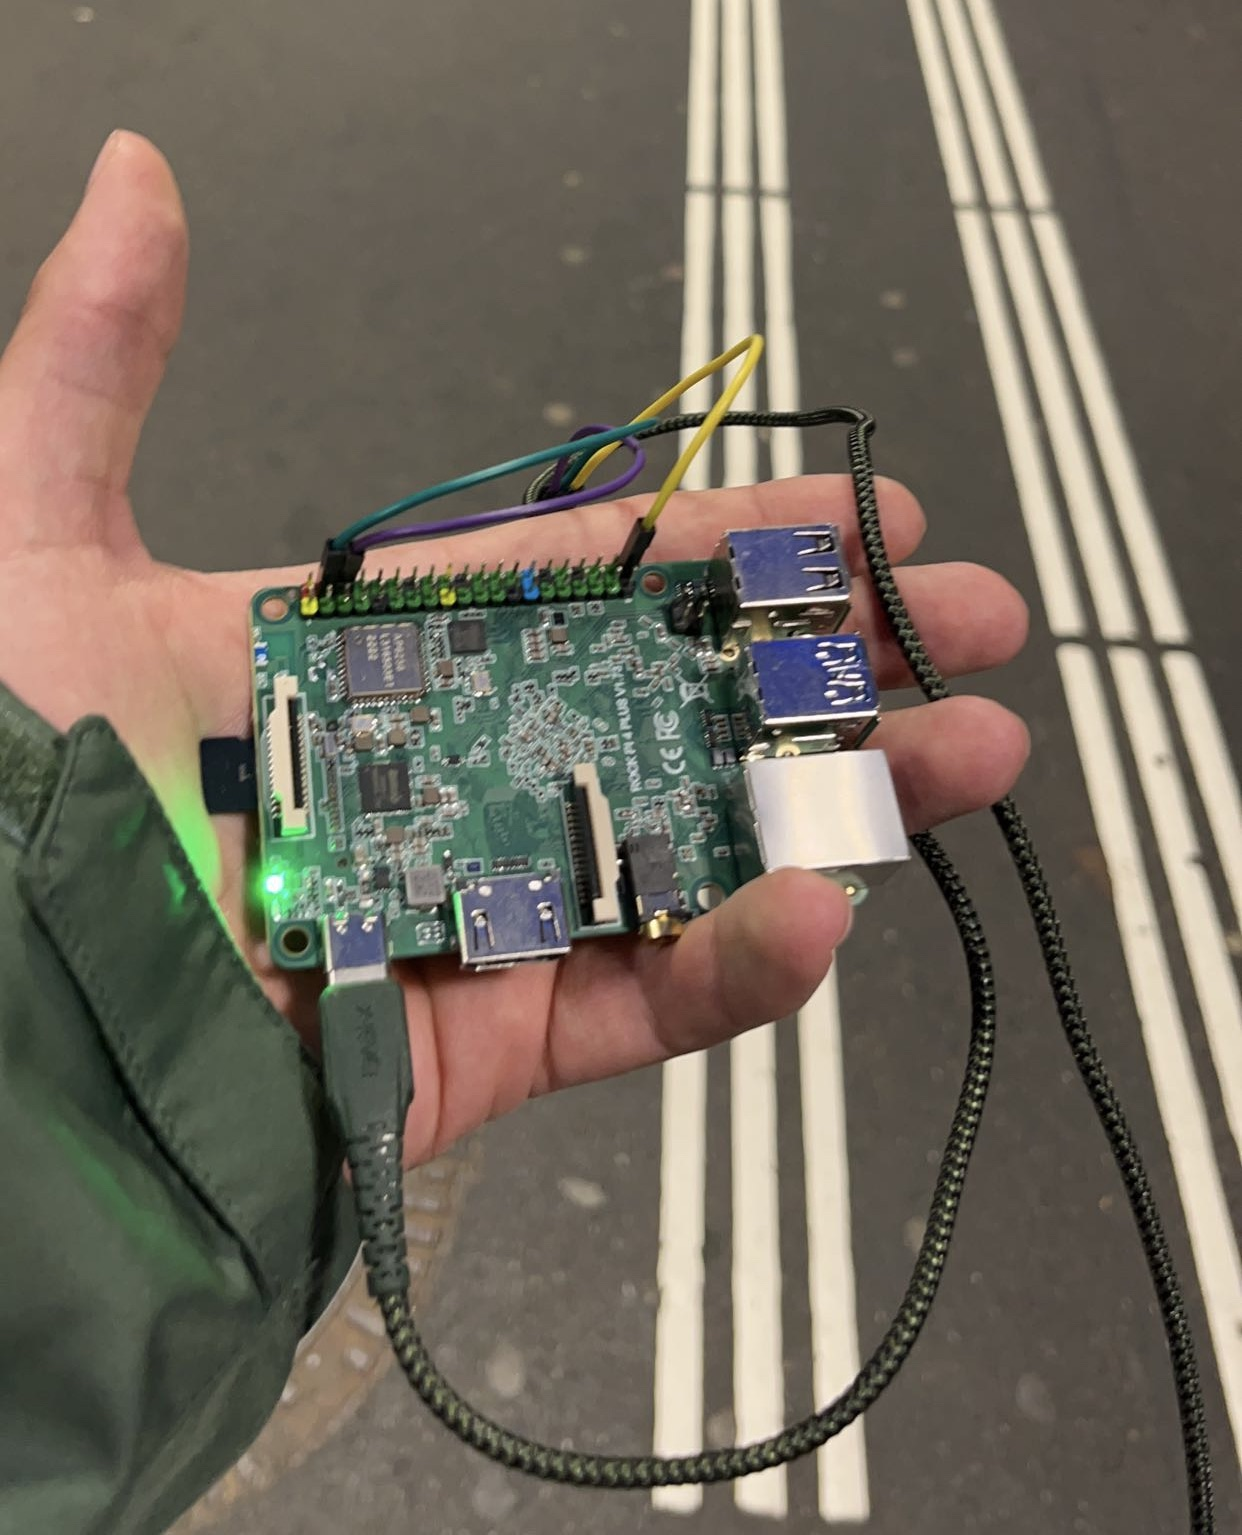
\includegraphics[height=0.25\textheight]{resources/field_test.jpeg}
        \caption{Simulating artwork transportation scenario}
        \label{fig:sensor_transport}
    \end{subfigure}
    \hfill
    \begin{subfigure}{0.5\textwidth}
        \centering 
        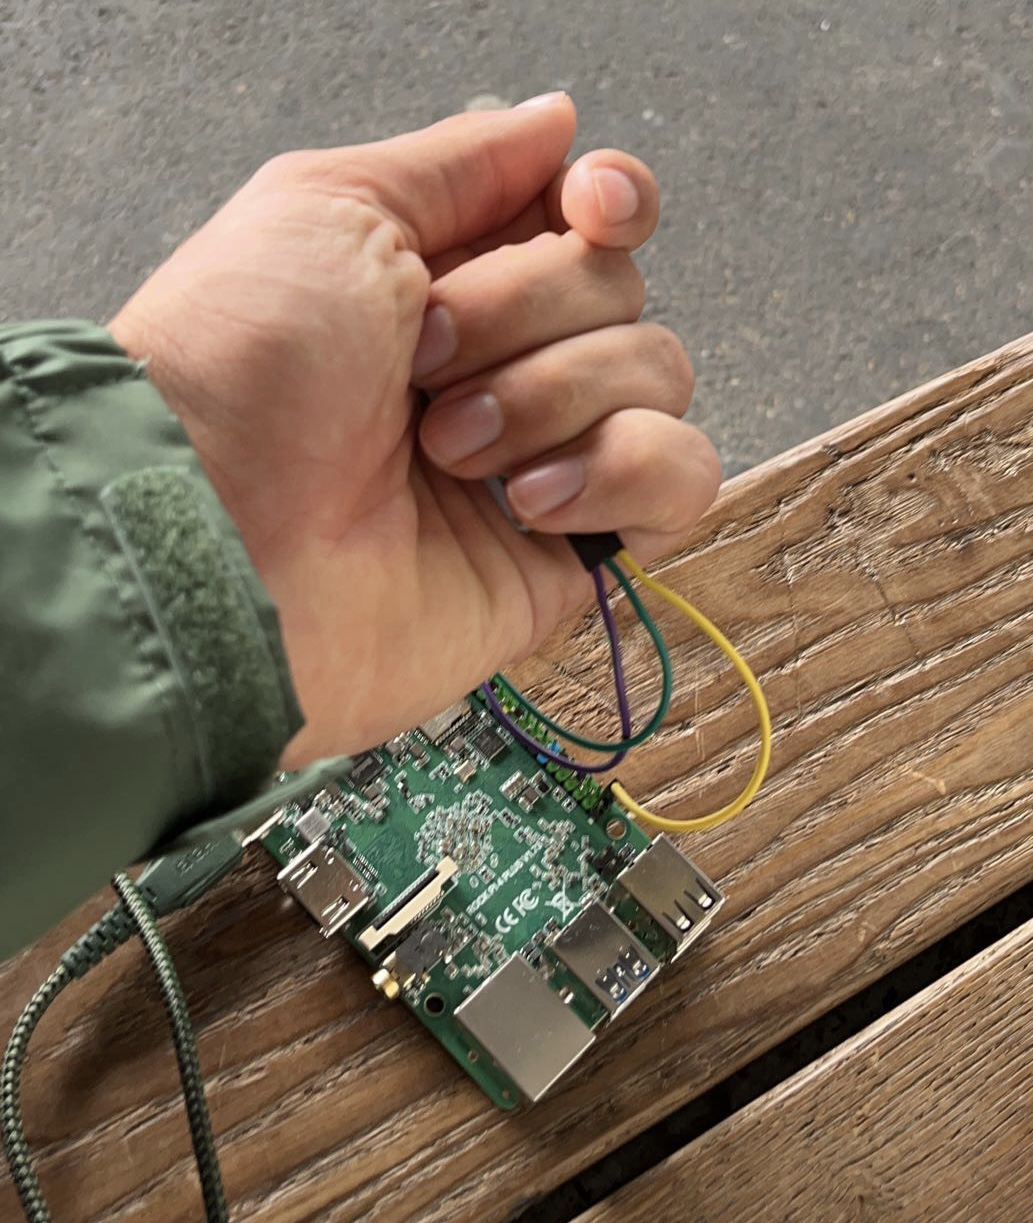
\includegraphics[height=0.25\textheight]{resources/cover_sensor.jpeg}
        \caption{Simulating temperature violation}
        \label{fig:covering_sensor}
    \end{subfigure}
    \caption{System Field Test}
    \label{fig:field_test}
\end{figure}

The field test involves a minimum of five requests to the \gls{api}. If any violations occur, this number is increased accordingly. We also simulated a temperature violation by covering the sensor with our hand (Figure \ref{fig:covering_sensor}) to include a violation in the test. The test was performed on the go, traveling by train and using a power bank to power the device and a hotspot from a cellular phone to connect to the internet. During the test, we recorded different metrics now used for evaluation. The most important metrics include a cost analysis of the field test and an evaluation of the performance of the logger.

\subsection{Cost}
During our field test, nine transactions were issued by the \gls{api}. The cost analysis also includes deploying the \gls{sc} and minting the \gls{nft}. However, this would be a one-time cost, and its significance will shrink with the number of transportation. Table \ref{tab:field_test_tx_fees} gives an overview of the transactions and estimated costs. The costs are estimated in the same manner as in Section \ref{sec:cost_and_performance}. However, the transactions were not issued with a fixed gas price, but each transaction was estimated based on the network at the time. 

The total cost of the field test mainly consists of the contract deployment. This transaction accounts for over 78\% of the total gas consumption and thus also accounts for the greatest cost factor. The variable part included in another similar transportation scenario of the same artwork amounts to around 25.85 \gls{chf} on the Ethereum network or around 0.05 \gls{chf} on the Polygon network.

\begin{table}[ht]
\centering
\begin{tabular}{lcc}
\multicolumn{1}{c}{\textbf{Transaction}} & \multicolumn{1}{l}{\textbf{Count}} & \multicolumn{1}{c}{\textbf{Total Cost on Ethereum (Polygon)}} \\ \hline
Contract deployment                      & one time                           & 143.79 (0.33)          \\
mint NFT                                 & one time                           & 12.05 (0.03)           \\
update status                            & 2                                  & 9.26 (0.02)            \\
approve status                           & 2                                  & 7.68 (0.02)            \\
report violation                         & 3                                  & 8.91 (0.03)            \\ \hline
\textbf{Total}                           & \textbf{9}                         & \textbf{181.69 (0.43)} \\
\hline
\end{tabular}
\caption{Transaction fees field test}
\label{tab:field_test_tx_fees}
\end{table}
\vspace{-0.5cm}
\subsection{Logger Reliability}
The field test lasted around 52 minutes. During the transportation, the logger stored every sensor reading in a local database. Figure \ref{fig:field_test_sensor_readings} illustrates the intervals of the sensor readings. Each line indicates a successful reading by the sensor; the red lines represent a violation. The maximum time between two readings was 9 minutes and 36 seconds. The shortest interval was less than a second. For this prototype, we did not test other metrics such as accuracy or range.

\begin{figure}[ht]
    \centering
    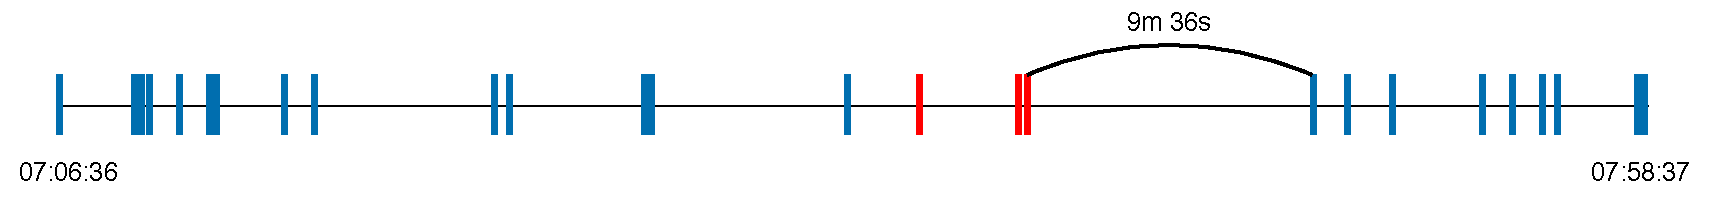
\includegraphics[width=\textwidth]{diagrams/sensor_eval.drawio.pdf}
    \caption{Timeline with sensor readings}
    \label{fig:field_test_sensor_readings}
\end{figure}


\section{Discussion}
\label{sec:eval_discussion}
The performance and cost of the developed system depend mainly on the blockchain used as infrastructure. The selection of such a blockchain thus is of significant importance and must be chosen with great diligence. The current prototype deployed on the sepolia testnet demonstrates the influence of different factors, such as network congestion and priority fees on the time needed for a transaction to be completed. On the testnet, the average response time with a fixed gas price of 30 Gwei is reasonable and could support a real-life scenario. However, this is not representative of the mainnet.

However, the gas consumption of the \gls{sc} functions can be directly adapted to any block-chain running the same \gls{evm} version. The analysis shows that executing a simple scenario on the Ethereum network can be very costly. Polygon presents a solution to this issue as our cost estimation is reduced by a factor of over 422. On Ethereum, the total cost of a scenario is quite costly, but considering the artwork's potential value, we think it could be acceptable for a real-life scenario. With Polygon, the estimated total cost is minimal and acceptable.

The security risks illustrated in Section \ref{sec:security_analysis} prevent the system from being used in a real-life artwork transportation scenario. The developed system serves as a proof of concept, and the security vulnerabilities must be mitigated for a production version.

The intervals of successful readings by the sensor have shown to be inconsistent and leave large gaps between readings. Unfortunately, the quality of the sensor would not be enough to support a real-life use case. A suitable sensor should be able to consistently record at shorter intervals preferably less than a minute long. The reason for the sensor's poor performance is unclear. Possible explanations include a timing issue in the communication between the board and the sensor, voltage fluctuations as the board was powered by a portable power bank or other environmental factors. We believe that this issue could easily be solved by using a higher quality board with integrated sensors such as the B-L462E-CELL1 Discovery kit by ST \cite{stmdevice}. 

